\documentclass[a4paper, 12pt]{article}

\usepackage{cmap} % поиск в PDF lusepackage[2A]{fontenc} % кодировка

\usepackage[utf8]{inputenc} % кодировка исходного текста
\usepackage[english,russian]{babel} % локализация и переносы
\usepackage{amsmath, amsfonts, amssymb, amsthm,mathtools, float}
\usepackage{ stmaryrd }

% Рисунки
\usepackage{graphicx}
\usepackage{wrapfig}

\usepackage[left=2cm,right=2cm, top=2cm,bottom=2cm,bindingoffset=0cm]{geometry}

\usepackage{longtable}
\graphicspath{pictures}

\author{Балдин Виктор Б01-303}
\title{Работа 1.1.4 \\ Измерение интенсивности радиационного фона}

\begin{document}

	\maketitle
	\section{Аннотация}
	\textbf{Цель работы:} применение методов обработки экспериментальных данных
	для изучения статистических закономерностей
	при измерении интенсивности радиационного фона.
	\bigskip\\
	\textbf{Оборудование:} счетчик Гейгера-Мюллера (CTC-6), блок питания, компьютер
	с интерфейсом связи со счетчиком.

	\section{Теоретические сведения}
	В данной работе измеряется число частиц, проходящих через счетчик за 10 секунд, с помощью которого мы можем найти и количество за 40 секунд. Такие времена выбраны для того, чтобы показать, что при большем времени лучше выполняется нормальное распределение измеряемых величин и гистограмма более симметрична, чем при малых временах, когда при оработке лучше воспользоваться законом Пуассона.

	Если случайные события, такие как регистрация частицы счётчиком, однородны во времени и являются независимыми, то результаты их измерений подчиняются распределению Пуассона. Теория вероятности утверждает, что в таком случае среднеквадратичная ошибка числа отсчётов, измеренного за некоторый интервал времени, равна квадратному корню из среднего числа отсчётов за тот же интервал:

	\begin{equation}
		\sigma = \sqrt{n_0}
	\end{equation}


		Для рассмотренной выборки из $n$ измерений относительная ошибка отдельного измерения равна:
	\begin{equation}
		\varepsilon_{\mbox{\tiny{отд}}} \approx \frac{1}{\sqrt{n_i}}
	\end{equation}
	При проведении многочисленных опытов за $n_0$ принимается среднее арифметическое всех результатов
	$\overline n$, а стандартная отклонение $\overline n$ от $n_0$ может быть
	вычислена по формуле:
	\[ \sigma_{\overline n} = \frac{1}{N} \sqrt{\sum_{i=1}^N(n_i - \overline n)^2}, \] где $N$ - количество измерений, $n_i$ - результат $i$-того измерения. Относительная же погрешность составит: \[ \varepsilon_{\overline n} = \frac{1}{\sqrt{\overline n N}}. \]


 	\section{Методика измерений}
	\begin{figure}[H]
		\centering
		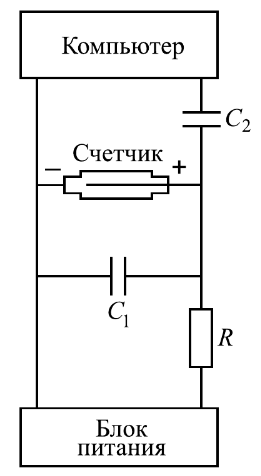
\includegraphics[scale = 0.5]{pictures/scheme.png}
		\caption{Схема включения датчика}
	\end{figure}
	
	Космические лучи обнаруживают с помощью ионизации, которую они производят, используя счетчик Гейгера-Мюллера. Схема его подключения приведена на рисунке 1. Счетчик представляет собой наполненный гахом сосуд с двумя электродами. Частицы космических лчей ионизируют газ, выбивают электроны из стенок сосуда. Те, сталкиваясь с молекулами газа, выбивают из них электроны. Таким образом, получается лавина электронов, следовательно, через счетчик резко увеличивается ток.


Измерения потока частиц с помощью счетчика Гейгера-Мюллера мала по сравнению с изменениями самого потока, то есть его флуктуациями.
	\section{Используемое оборудование}

	\section{Результаты измерений и обработка данных}
	\section{Обсуждение результатов}
	\section{Вывод}
\end{document}
